\begin{figure*}
\centering
\begin{minipage}{0.48\textwidth}
\centering
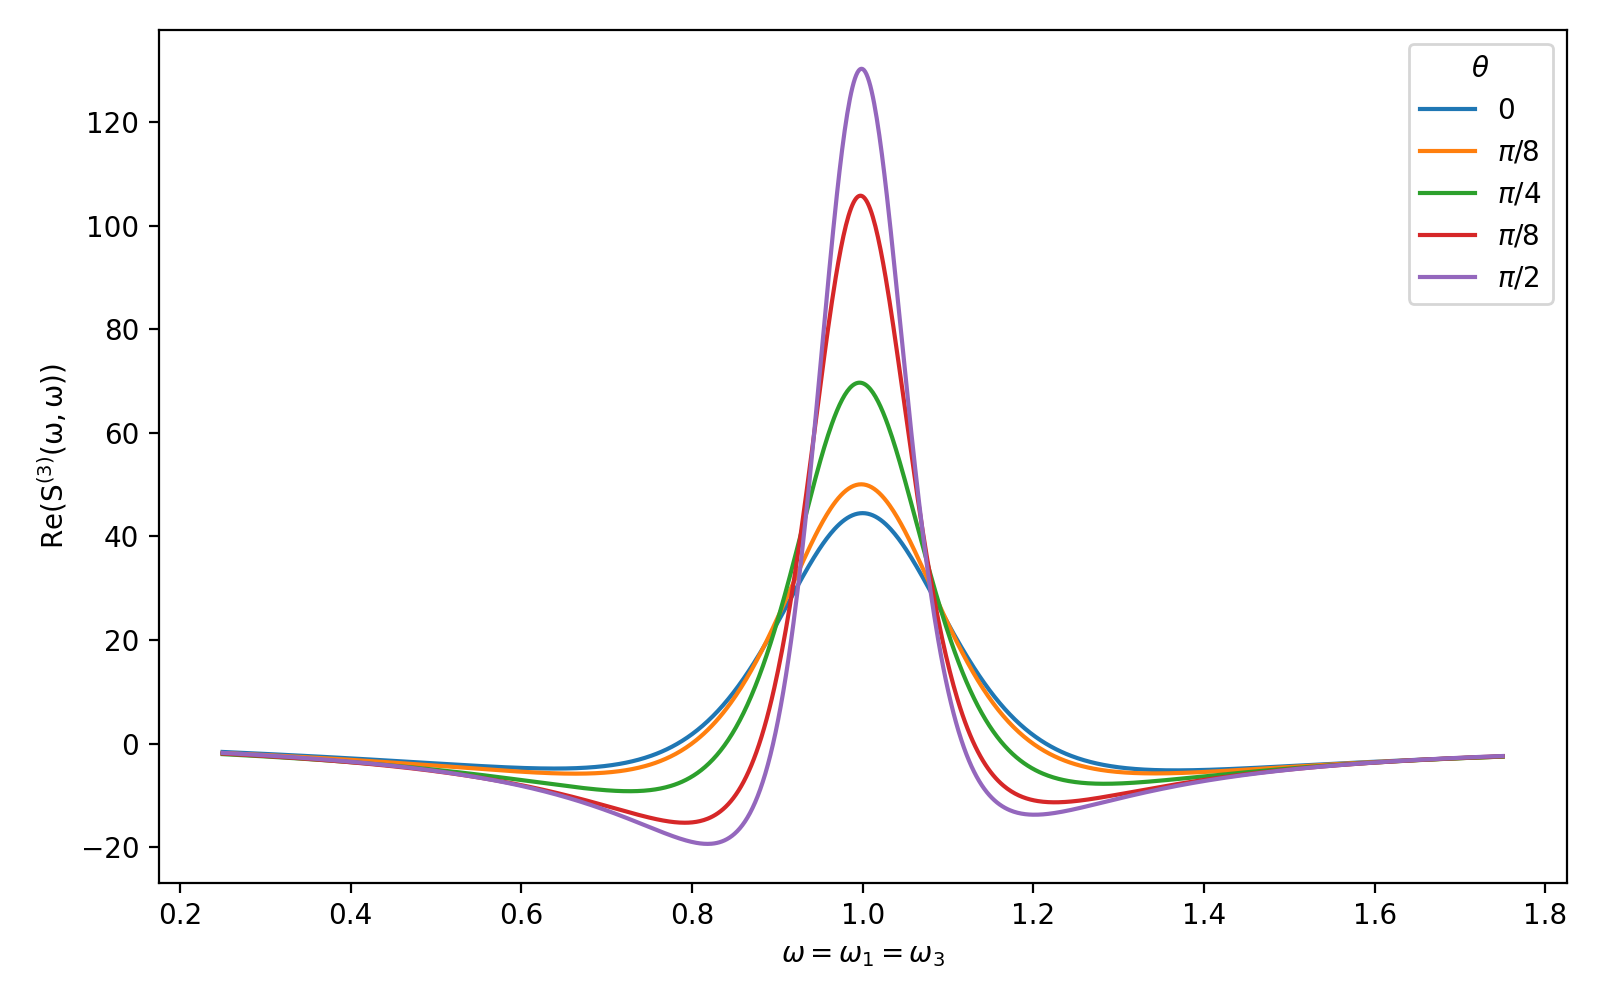
\includegraphics[width=\linewidth]{Figures/corrected_diag_theta_real_2.png}
\end{minipage}
\hfill
\begin{minipage}{0.48\textwidth}
\centering
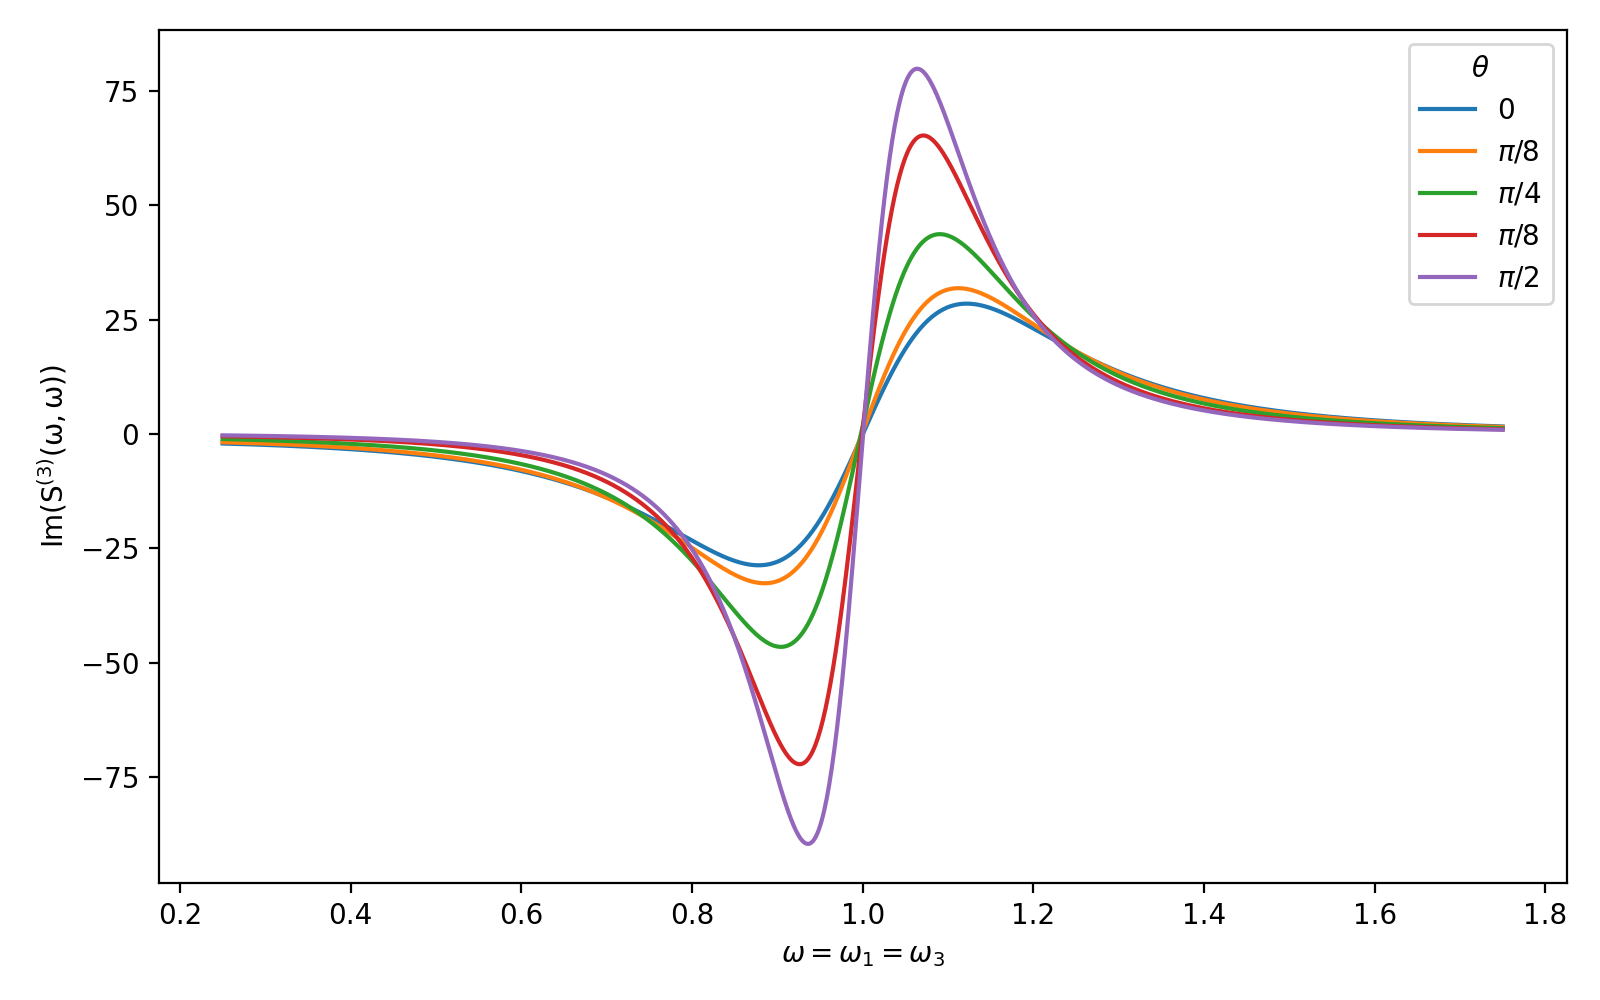
\includegraphics[width=\linewidth]{Figures/corrected_diag_theta_imag_2.png}
\end{minipage}
\caption{Real (left) and imaginary (right) components 
of the diagonal spectral response for increasing 
pointer-basis misalignment $\theta$. At $\theta = 0$, 
only dephasing contributions are present. For 
$\theta \neq 0$, basis misalignment mixes response 
pathways, producing continuous and structured 
deformations of the complex spectrum. These serve 
as benchmarks for the Duhamel reconstructions shown 
in Fig.~\ref{fig:TransportError}.}
\label{fig:DiagResponse}
\end{figure*}